\documentclass[conference,9pt,letterpaper]{IEEEtran}
\usepackage{amsmath,amssymb,graphicx,booktabs,array}
\usepackage{flushend}
% Compact float spacing for final-column mechanism details.
\setlength{\textfloatsep}{6pt plus 2pt minus 2pt}
\setlength{\intextsep}{6pt plus 2pt minus 2pt}
\setlength{\floatsep}{6pt plus 2pt minus 2pt}
\usepackage{fontspec,unicode-math}
\setmainfont{NimbusRoman-Regular.otf}[BoldFont=NimbusRoman-Bold.otf,ItalicFont=NimbusRoman-Italic.otf,BoldItalicFont=NimbusRoman-BoldItalic.otf]
\setsansfont{NimbusSans-Regular.otf}[BoldFont=NimbusSans-Bold.otf,ItalicFont=NimbusSans-Italic.otf,BoldItalicFont=NimbusSans-BoldItalic.otf]
\setmathfont{Latin Modern Math}
\setlength{\dbltextfloatsep}{6pt plus 2pt minus 2pt}
\setlength{\abovecaptionskip}{5pt}
\usepackage[hidelinks]{hyperref}
\hypersetup{pdftitle={LoDA-SA: Low-Frequency Distance-Aware Two-Level Sparse Attention},pdfauthor={},pdfsubject={Near--far two-level sparse attention with shared low-frequency RoPE coordinates},pdfkeywords={},pdfcreator={LaTeX}}
\newcommand{\Top}{\operatorname{TopK}}
\newcommand{\clip}{\operatorname{clip}}
\graphicspath{{../figures/}}
\title{LoDA-SA: Low-Frequency Distance-Aware Two-Level Sparse Attention}
\author{\IEEEauthorblockN{Anonymous authors}}
\begin{document}
\maketitle
\begin{abstract}
Sparse attention must retain useful candidates at low selection cost. We study LoDA-SA, a distance-aware two-level selector: a near--far page-to-token cascade with shared 32-coordinate low-frequency RoPE scoring, original-dimensional attention on selected tokens, and absolute budgets: protected sink and window lengths, a near extent, a near page quota with far pages by subtraction, and one free-competition token pool. Ratio-coupled parameterizations instead silently reallocate far capacity: one expression links the far token budget to three knobs, and archived diagnostics exhibit all three failures, including an exact integer threshold. The absolute interface makes page capacities explicit and drops regional token quotas. An 87-cell grid on five LongBench tasks (Qwen3-8B) attributes quality to near pages and near extent, finds no token-split main effect, and averages 48.26 for quota-free selection at 32 near pages and 4096-token extent versus 47.46 for a no-partition control; archived RULER 32K runs reach 59.29. These single-run comparisons establish neither non-inferiority nor mechanisms; historical timings show slower sparse decoding, and the compact 4/128 design still requires matched quality and preparation-inclusive complete-request cost.

\end{abstract}
\begin{IEEEkeywords}
sparse attention, shared representation, regional retrieval, long-context inference
\end{IEEEkeywords}

\section{Introduction}
In dense long-context decoding, each new token attends to a growing history of cached keys and values. Sparse attention restricts final attention to selected tokens, but selecting them requires scoring, ranking and memory accesses. The design goal is to preserve task-relevant tokens within a fixed budget while keeping selection cheaper than the attention work it removes. Both candidate selection and final attention-set size are central design problems.

Cascades such as AsyncTLS shortlist pages using inexpensive summaries before token refinement~\cite{asynctls}. Mean pooling and sign-aware extrema, summaries our selector also uses, do not rank pages by their total attention weight. Following ClusterKV's token/page perspective~\cite{clusterkv}, Figure~\ref{fig:observation}(a) shows a single Qwen3 query where fewer missed mass-ranked reference pages coincide with more missed reference-page mass. Unequal regional allocations and realized counts preclude a controlled comparison but motivate examining how scoring and budgets shape candidate access.

The two summaries fail in opposite regions. Across 128 correlated observations (Fig.~\ref{fig:observation}(b)), block averaging misses .084 of near reference mass and .170 of far reference mass; sign-aware extrema miss .079 near and .042 far. Near misses are on par (.084 versus .079); far misses differ fourfold (.170 versus .042), because page averages dilute sparse far spikes while extrema lose their advantage on uniform near mass. No split of the 2048-token budget beats global extrema selection on this diagnostic plane, so budget division is a task-accuracy question.

We study a two-level selector that couples a shared scoring view with absolute regional budgets. Both stages use a fixed set of 32 coordinates comprising 16 complete low-frequency RoPE pairs; near pages receive an explicit integer quota with far pages by subtraction, the near extent is absolute, and L2 refines tokens in a single free-competition pool. Among the three 32-coordinate subsets in Figure~\ref{fig:observation}(c), low-frequency pairs retain .84 of full-dimensional reference mid-TopK mass on average, random coordinates .51, high-frequency pairs .24; the random subset does not preserve RoPE pairs. Selected tokens use original-dimensional Q/K/V in one final attention operation. Compact coordinates narrow each scoring dot product, but ordinary L2 still scores the full history before masking; fewer shortlisted pages do not remove that work. We also formulate a prefill-informed far gate motivated by layer variation in Figure~\ref{fig:observation}(d); it is disabled by default and requires separate evaluation.

We contribute LoDA-SA, an absolute-budget two-level selector with shared low-frequency coordinates, a unified analysis of implicit budget coupling in ratio parameterizations, an 87-cell grid isolating near pages and near extent as the active quality axes, and separate evaluations of task quality, regional coverage and execution cost. Under the archived ratio interface, one expression in the page cap, near share and fill fraction determines the far token budget, so raising any of the three can zero it; reported Qwen3-8B RULER 32K AVG moves 0.99 points when archived near quotas shift (16,640) to (8,320), with both quotas changing together. Grid cells are single runs, and the archived sparse configuration decodes slower than dense at every measured length. Establishing a quality--latency benefit for the compact design requires matched quality and complete-request measurements including preparation, maintenance and selection.

\begin{figure*}[t]\centering
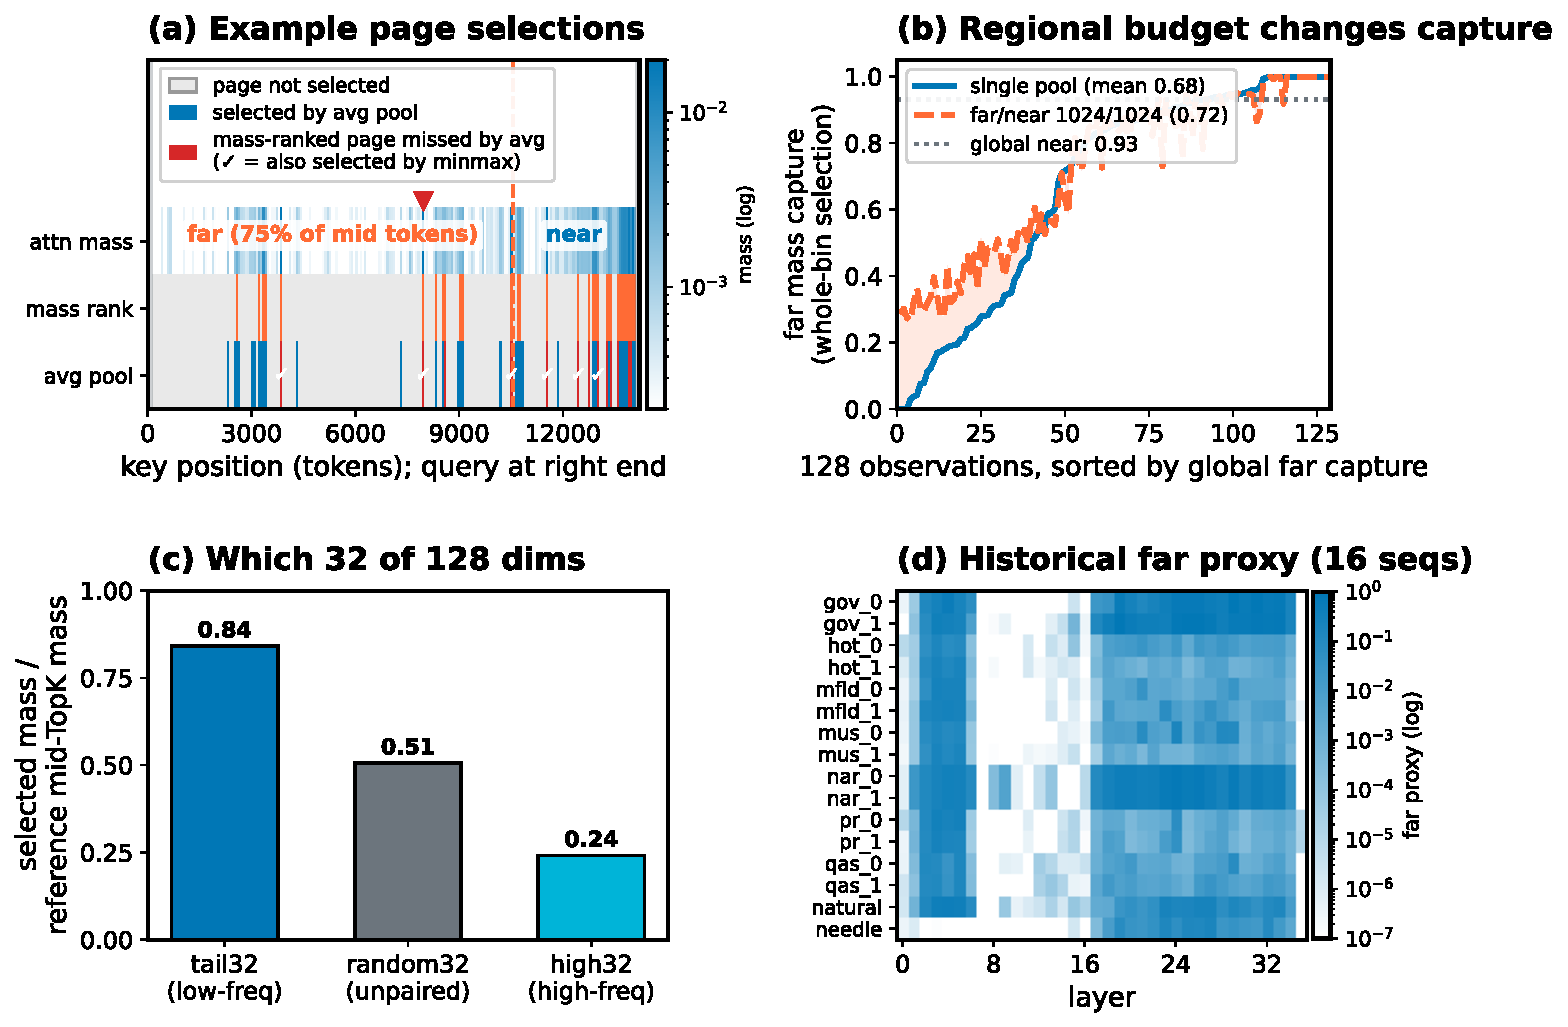
\includegraphics[width=\textwidth]{o_observation.pdf}
\caption{Four motivating diagnostics; Qwen3-8B, 128/128 prefix/recent protection in (a)--(c). (a) MuSiQue sample~1, layer~24, query~14212. The top strip shows summed attention per page, not a selection. Below: stored mass-rank, avg and minmax selections, 32 pages each, using 1989/1989/2048 tokens under a 2048 cap. Avg/minmax miss 13/17 reference pages holding 59.65\%/26.46\% of reference-page mass. Blue: selected reference pages; red hatching: missed reference; orange dots: selected outside the reference. Shaded spans mark the far and near regions. Mass-rank is a whole-page comparison reference, not an optimal oracle, exact token TopK or DSA. Avg and minmax share 32 coordinates and head aggregation; the reference uses full-dimensional attention weights. Different regional allocations and realized counts preclude inferring near/far specialization or task quality from these misses. (b) Missed reference mass by page region, mean over 128 correlated observations from four sequences: avg misses .084 near and .170 far, minmax misses .079 near and .042 far; averages dilute sparse far spikes, extrema lose on uniform near mass. Regions use absolute page intervals; no budget split beats global minmax on this plane. (c) Selected mass relative to full-dimensional reference mid-TopK mass; random32 does not preserve RoPE pairs. (d) One 16-by-36 historical single-query proxy matrix gives 24/36 layer medians below .01 and 12--32 low-proxy layers per sequence. It uses the last sampled query, group-logit summation before softmax and far interval $[64,t-2048)$ (S6), unlike the current gate. These are diagnostic selections and profiles, not task-quality or decode-safety results.}
\label{fig:observation}\end{figure*}

\section{Related Work}
Quest supplies sign-aware page-extremum bounds for far-page scoring, SparQ approximates attention from query-selected key coordinates, and HISA prunes the attention set hierarchically~\cite{quest,sparq,hisa}; SparQ protects a recent-token window, and HISA forces first and last blocks into its coarse candidate set. AsyncTLS already combines a page-to-token cascade with coordinate selection, quantization, per-query normalization followed by grouped-query-attention (GQA) probability aggregation, and final attention over original KV~\cite{asynctls}. Rather than proposing a new cascade, we study these existing components with complete low-frequency RoPE pairs shared across both stages and absolute near--far budgets, distinguishing page-level eligibility from final token capacity.

The selector's own reads also matter. Token-Picker uses conservative probability estimates from partial key-bit chunks to stop further key-chunk and value transfers for pruned tokens~\cite{tokenpicker}; our selector instead ranks candidates with a fixed coordinate subset under page budgets, keeping original-dimensional KV. Our selector keeps both selection stages in bf16: AsyncTLS token keys are INT4, FFD scans 2-bit keys, and official HISA pools block summaries in FP8~\cite{asynctls,ffd,hisa}; our efficiency comes from candidacy structure, regional quotas and page-level narrowing, not numeric compression. KV compression and placement methods address complementary storage and movement constraints~\cite{shadowkv,million,clusterkv}; a smaller scoring view retains original-KV capacity without lowering complete-request latency.

\section{Near--Far Selection in a Shared Subspace}
To control both selection cost and candidate access, the cascade uses two explicit mechanisms: a shared scoring view and absolute regional budgets. One 32-coordinate map supports both L1 page screening and L2 token refinement, separating low-dimensional selection from original-dimensional attention (Fig.~\ref{fig:architecture}). The cascade operates only during decoding; prefill remains dense. L1 assigns separate near and far page quotas, so neither region's pages compete for the other's allocation. Ordinary L2 scores the full history, applies the retained-page mask, then fills one free-competition token pool; selected indices merge with protected positions for attention using the original Q, K and V, and recomputing retained logits does not recover omitted tokens.
\begin{figure*}[t]\centering
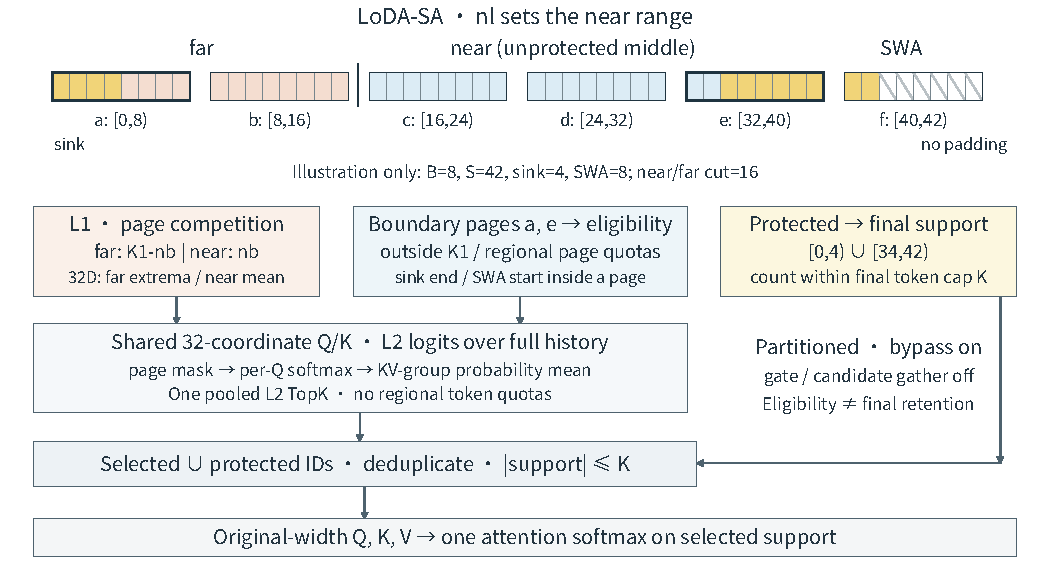
\includegraphics[width=\textwidth]{architecture_domains/fig2_domains_en.pdf}
\caption{Architecture of shared-subspace selection, with the optional gate inactive. A shared coordinate view feeds regional L1 page scoring and ordinary full-history L2 scoring. Page masks limit eligibility; per-query softmax and KV-group probability averaging precede single-pool token selection. Protected positions join deduplicated IDs within $K$. Near excludes the protected recent window. IDs define support over original-width K/V; physical gathering is backend-dependent. Original Q follows a separate path. Arrays are schematic.}
\label{fig:architecture}\end{figure*}

\subsection{Shared low-frequency coordinates}
Both regions and both selection stages use the same coordinate map within each layer and KV head, while each query head is scored separately. For Qwen3-8B, we select post-RoPE coordinates $J=\{48,\ldots,63,112,\ldots,127\}$ from each 128-dimensional query and key. The indices retain 16 complete low-frequency split-half RoPE pairs (Supplementary Fig.~S1). With coordinate-selection matrix $E_J\in\mathbb R^{128\times32}$, the scoring vectors are $z_q=E_J^\top q$ and $z_i=E_J^\top k_i$. The retained pairs' slow positional rotation motivates this selection, although it does not guarantee preservation of important tokens. The compact implementation uses width-32 scoring tensors, whereas the historical quality runs used 32 active coordinates in width-128 L2 tensors (S7).

L1 aggregates selected key coordinates into page summaries for coarse ranking; L2 refines candidates with per-token scores in the same coordinate view. Original KV remain full width. Compact scoring narrows each dot product fourfold, but view preparation and maintenance add work without compressing the original KV cache (S7).



\subsection{Absolute budgets and regional eligibility}
In decoding, $t$ indexes the current token from zero across the full sequence including prefill. Let $s$ and $w$ denote the protected sink and recent-window lengths, with protected set $\mathcal P_t=\{i:0\le i\le t,\ i<s\ \text{or}\ i>t-w\}$ and unprotected middle $\mathcal M_t=\{0,\ldots,t\}\setminus\mathcal P_t$; overlapping protection counts once. Near is a suffix of $\mathcal M_t$ with explicit page-aligned extent $L_n$ (whole middle when shorter); far is the rest. Near excludes the protected recent window.

Regional page caps constrain L1 eligibility (Supplementary Fig.~S2). Near pages use query--mean-key dot products to summarize page-level relevance; far pages use sign-aware extrema to bound shared-space token scores, a heuristic assignment. Summaries cover full physical pages including protected boundary positions; L2 separately limits token regions (S7). For a nonempty page $b$, let $m_{b,j}=\min_{i\in b}z_{i,j}$ and $M_{b,j}=\max_{i\in b}z_{i,j}$. Quest's construction~\cite{quest} gives
\begin{equation}
U_b(z_q)=\sum_j\bigl(z_{q,j}^{+}M_{b,j}+z_{q,j}^{-}m_{b,j}\bigr),
\label{eq:bound}
\end{equation}
where $z^+=\max(z,0)$ and $z^-=\min(z,0)$. Each signed coordinate contribution is bounded by its chosen extremum, so $z_q^\top z_i\leq U_b(z_q)$ for every shared-space key in $b$. This does not bound original-dimensional logits. Extrema may come from different tokens, making the bound loose enough to misrank pages and miss important tokens. Average-key scores lack this per-token bound.

For total cap $K\geq|\mathcal P_t|$, the middle-token budget $K_{\mathrm{mid}}=K-|\mathcal P_t|$ fills one pool: L2 applies the retained-page mask, then a single TopK over group-averaged probabilities retains up to $K_{\mathrm{mid}}$ tokens regardless of region. The interface exposes absolute quantities: near page quota $n_p$, far pages $K_1-n_p$ by subtraction, and near extent $L_n$. Each is explicit; neither region's page capacity moves without its own parameter. With enough positive-probability candidates, L2 cannot recover unprotected tokens from L1-rejected pages. S7 details scarce-support and masked zero-tie exceptions.

Ratio-coupled interfaces hide this subtraction. The archived parameterization derives $n_p=\max(1,\operatorname{round}(\beta K_1))$ and $n_k=\min(\lfloor\gamma n_pB\rfloor,K_{\mathrm{mid}})$ with ties-to-even rounding, so the far token budget reduces to
\begin{equation}
k_f=\max\bigl(0,\,K_{\mathrm{mid}}-\min(\gamma n_pB,\,K_{\mathrm{mid}})\bigr).
\label{eq:coupling}
\end{equation}
Three knobs, $K_1$, $\beta$ and $\gamma$, therefore reallocate far capacity through one expression, while far pages remain admitted at $k_f=0$: page eligibility and token capacity are separate constraints. Archived diagnostics exhibit all three reallocations, including an exact integer threshold at which raising $K_1$ zeroes far tokens (Q2, S6). The absolute interface is immune by construction: the single token pool is stated, not derived, and no knob combination can zero a region's token access.

With disjoint protection and sufficient candidates, the compact configuration ($K=1024$, $s=4$, $w=128$, $n_p=32$, $L_n=4096$) leaves 892 middle slots per KV head, with L1 admitting 32 near and 96 far pages (Supplementary Fig.~S2). The partial prefix page can reselect up to four protected tokens, so retained coverage is nominal.



\subsection{GQA selection and original-dimensional attention}
GQA assigns four of Qwen3’s 32 query heads to each of its eight KV heads. L1 averages their page scores before regional TopK. Ordinary L2 computes each query’s full-history logits, applies the shared page mask, then softmax. Group-averaged probabilities determine the single-pool token TopK. L2 uses scale $1/\sqrt{128}$ before softmax even with 32 scoring coordinates. Because softmax precedes group averaging, this rule generally differs from applying softmax to group-averaged logits. A smaller L1 shortlist restricts eligibility without reducing ordinary L2's full-history dot products.

For KV group $h$, let $\mathcal S_{t,h}$ be the deduplicated union of protected positions and regional winners, with $|\mathcal S_{t,h}|\leq K$. Each query $g$ uses this support for its own full-dimensional attention ($d=128$):
\begin{equation}
o_{h,g}=\sum_{i\in\mathcal S_{t,h}}\frac{e^{q_{h,g}^{\top}k_{i,h}/\sqrt d}}
{\sum_{j\in\mathcal S_{t,h}}e^{q_{h,g}^{\top}k_{j,h}/\sqrt d}}v_{i,h}.
\end{equation}
Each query applies one softmax over the merged indices, avoiding the addition of separately normalized regional outputs~\cite{salo}. Full-dimensional retained logits still use a restricted denominator, which can change the output. Physical KV gathering and reuse depend on backend and length; short sequences can use a dense masked path.

\subsection{Prefill-informed far gating}
The optional gate, disabled by default, exploits layer variation: layers whose mean prefill far-attention proxy falls below $\epsilon$ skip far selection, and the first decode-path call freezes the decision until input reset (Supplementary Fig.~S3; S5). OFF skips far L1/L2 scoring and selection; the single pool then draws only from retained near pages, whose L1 cap stays unchanged; removing far support can still change softmax denominators and group-averaged near rankings. Calibration uses a token-defined region that can differ from the page-aligned skipped region, the threshold does not bound decoding error, and preparation, sequence-wide buffers and normalization remain (S5).



\begin{figure*}[t]\centering
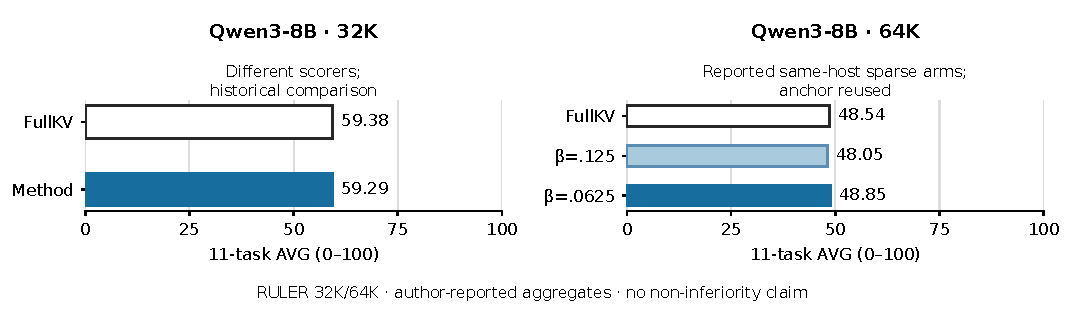
\includegraphics[width=\textwidth]{ruler32k_comparison/ruler32k_avg_compact_en.pdf}
\caption{Author-reported RULER 32K/64K AVG on Qwen3-8B: 11 tasks, 100 examples/task/arm. FullKV is dense; archived sparse arms report $K=1024$, protection 4/128 under ratio-derived token quotas, predating the selected free-competition configuration. At 32K, near quotas (8,320) ($\beta=.0625$); at 64K, (8,320) and (16,640) are both shown. The 32K comparison spans machines (scorers differ, input identity partial); the 64K sparse arms are reported on one machine, the FullKV anchor a separate run. Gate status and scoring dimensions are unverified. These descriptive scores establish neither non-inferiority nor matched quality--cost benefit (S8).}
\label{fig:ruler32k-quality}\end{figure*}

\section{Experimental Setting}
We evaluate three aspects separately: task quality (Q1), regional candidate coverage (Q2) and execution cost (Q3). Table~\ref{tab:settings} defines the compact Qwen3-8B design: dense prefill, sparse decoding and a 1024-token cap including four prefix and 128 recent tokens (the 4/128-protection design). We selected $n_p$ and $L_n$ from an 87-cell LongBench grid (Q2), whose token-split axis shows no main effect; L2 fills $K_{\mathrm{mid}}$ by free competition, the archived $\gamma$-off mode. Archived runs use ratios $(\alpha,\beta,\gamma)$ mapping to the same geometry via $n_p=\max(1,\operatorname{round}(\beta K_1))$, $n_k=\min(\lfloor\gamma n_pB\rfloor,K_{\mathrm{mid}})$ and page-aligned $L_n=\lfloor\alpha|\mathcal M_t|\rfloor$; $(8,320)$ equals the archived $(.25,.0625,.625)$ cell (S7). Archived quality runs applied 16-level quantize--dequantize to L2 token keys, an implementation detail outside the mainline (S7). The historical five-task LongBench shared-subspace arm uses an earlier implementation: 128/128 protection and 32 active coordinates in zero-filled width-128 L2 keys. The labels ``full-dimensional page/token scoring'' denote reported variants without complete execution configurations, not controlled single-stage ablations. Synthetic selector and model-level decode timings come from separate studies without matched quality or cost (S6/S7).
\begin{table}[t]\centering\small
\caption{Compact design parameters and execution policy. These settings define the proposed implementation, not the historical runs. $K$ includes unique protected tokens.}\label{tab:settings}
\begin{tabular}{ll}\hline
Parameter & Setting \\\hline
Final token cap $K$ & 1024 \\
Page size; L1 page cap $K_1$ & 64; 128 \\
Near page quota $n_p$ (far) & 32 (96) \\
Near extent $L_n$ & 4096 tokens, page-aligned \\
L2 token selection & single pool, free competition \\
L1/L2 active coordinates & 32/32 \\
Prefix / recent protection & 4/128 \\
Prefill; decode layers & dense; all sparse \\\hline
\end{tabular}\end{table}

\textbf{Workloads and comparisons.} Reported quality covers five-task LongBench~\cite{longbench} and 11-task RULER~\cite{ruler} (Qwen3-8B: 32K/64K, historical 128K), plus ported Quest/AsyncTLS/JSSA baselines. Three nominal sparse LongBench variants lack verified factorial isolation. FullKV is dense and uncapped (RULER/decode timing). Method comparisons must disclose native prefill/decode paths; policy-matched adaptations need separate reporting. Budget matching aligns final unique-token caps $K$ including protection; realized counts and head sharing affect KV traffic, and equal $K$ alone establishes neither (S7).

\textbf{Metrics.} Primary quality is task-score AVG over each fixed benchmark/length set; per-task gains and losses explain AVG without zero-loss requirements. Policy-matched controls require matched models, samples, lengths, scorers, phase policies and aligned sparse-token budgets; incomplete sets lack full-set AVG. Regional miss shares divide missed reference mass by page region (Fig.~\ref{fig:observation}(b)); panel (c) normalizes by full-dimensional mid-TopK mass. Neither selector time (synthetic single-layer) nor synchronized TPOT (model-level post-first-output intervals) measures preparation-inclusive complete-request latency, so unpaired studies define no quality--latency frontier; AVG differences are descriptive, not non-inferiority evidence.

\begin{figure}[t]\centering
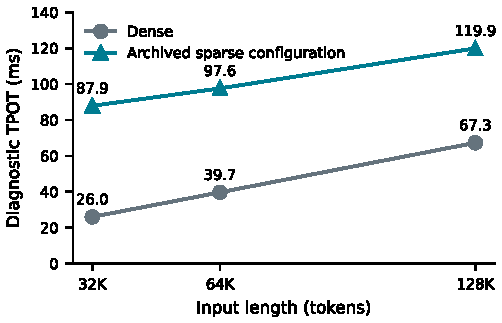
\includegraphics[width=\columnwidth]{decode_tpot_current.pdf}
\caption{Author-reported model-level decode TPOT for an archived sparse configuration and dense FullKV, Qwen3-8B with dynamic cache. Fixed 128-token output gives 127 after-first intervals, including synchronization and argmax. The archived $(.125,.375,.625)$ setting differs from the selected 4/128 candidate; these medians measure no complete-request E2E and establish no matched quality--cost comparison (S6).}
\label{fig:pending-evaluation}\end{figure}

\section{Evaluation and Discussion}
\subsection{Q1: Does reduced scoring width preserve task quality?}
On HotpotQA, Qasper, MuSiQue, GovReport and RepoBench-P~\cite{longbench}, five-task means fall within a 0.33-point spread: shared-subspace 47.588, the nominal page variant 47.910 and the token variant 47.666 (Supplementary Fig.~S4). These differences describe recorded configurations, not evidence that reduced width preserves quality: the variants are not verified single-factor interventions, and the shared-subspace run uses earlier 128/128 protection. All three arms are sparse; dense FullKV is a different reference.

\subsection{Q2: How do regional budgets constrain candidate access?}
\textbf{Grid-isolated axes.} An 87-cell absolute-quota grid (Qwen3-8B, five LongBench tasks, one run per cell) sweeps near pages, near extent and the token quota. A no-partition control averages 47.46; free competition at $(n_p,L_n)=(32,4096)$ averages 48.26, the best quota-free cell 48.30. Near-page marginal means rise monotonically from 46.37 to 48.21 and flatten at 64, and best cells cluster near $n_pB\approx L_n/2$, matching near-region mass concentration (top-half pages hold a median .93). The token quota shows no main effect: it beats free competition by a mean of .04 across 69 cells (42/69 positive), so the design drops the split; the best quota cell exceeds the best quota-free cell by .37, and top-3 paired bootstrap intervals contain zero (S6).

Archived RULER 32K arms move 58.30$\rightarrow$59.29 as near quotas shift $(16,640)\rightarrow(8,320)$ (archived $\beta=.125\!\rightarrow\!.0625$), with far pages and far tokens rising jointly; the near-page-4 arms score 58.07 ($K_1=128$) and 58.96 ($K_1=256$), both below $(8,320)$. These archived ratio-interface runs are not the selected configuration; records match, predictions unreplayed.

\textbf{Implicit coupling failures.} Archived diagnostics exhibit all three reallocations of Eq.~(\ref{eq:coupling}). Integer enumeration of the archived formulas locates the first far-zero page cap at $K_1=156$ for $K=1024$ ($B=64$, $\beta=.125$, $\gamma=.625$, 128/128 protection); far budget 8 remains at $K_1=155$, so capacity appears to grow while far tokens vanish. Archived task scans collapse HotpotQA from 53.6--57.3 to 37.7 exactly on zero-far-budget arms, graded by far fraction (16.4 points at .875, about 1 at .125). At the archived grid cell $(\alpha,\beta)=(.25,.125)$, free competition ties the best $\gamma$ within .001 in retained-mass diagnostics (.852 versus .8515), while $\gamma=0$ reads as far-free but zeroes the near token quota, dropping retained mass to .827. These archived diagnostics unify the three anomalies but are not new controlled experiments.

Reported 32K AVG gap to dense FullKV is $-0.09$ across machines; at 64K, AVGs are 48.85/48.05 for near quotas (8,320)/(16,640) versus 48.54. Sparse arms share a machine and scorer hashes but differ in prediction scripts; the dense anchor differs in scorer and identity, and missing paired intervals preclude causal conclusions (S8).

\textbf{Ported baselines.} Author-reported AVGs (nominal 512): 56.00 (ours) and 48.33 (AsyncTLS), a reported 7.67-point gap; AsyncTLS/FASA artifacts sit outside the repository snapshot, and unique-token/protection/phase matching is unverified. At $K=1024$, 59.29 compares with JSSA's 58.7 (nominal 1024), Quest's 42.85 and FASA's 18.64; $K=384$ scores 15.00. S8 gives provenance, CWE's 43.4-point loss and absent paired intervals.

At 128K, the (8,320)/(16,640) arms score 45.73/46.02 on one machine; 45.73 is 98.49\% of the separate-run dense anchor, 46.43. Historical RULER 128K yields 23.98 (sparse) under budgets implying $k_f=0$, execution unverified, the 22.45-point loss unexplained (S6). Five-task LongBench means are 26.09 (protection-only, 256 tokens) versus 47.91 (reused sparse, 1024); retrieval and budget both change.

\subsection{Q3: Does compact scoring reduce execution cost?}
\textbf{Model-level decoding.} The reported sparse configuration is \mbox{slower} than dense FullKV at every measured length (Fig.~\ref{fig:pending-evaluation}). \mbox{Sparse} TPOT medians are 87.9, 97.6 and 119.9 ms at 32K, 64K and 128K, compared with dense medians of 26.0, 39.7 and 67.3 ms. The relative penalty shrinks with length, but absolute sparse TPOT increases: no decode-time benefit. Timings include synchronization and argmax, use a non-compact configuration, and cannot locate causes or predict the compact implementation (S6).

\textbf{Local selector cost.} A separate two-round synthetic experiment (single layer, batch one, one query, 64K QKV) reports steady-state summaries of 1.3502, 1.3598 and 1.4634 ms (full-dimensional page, shared-subspace, token variants); shared-subspace runs 0.0237 ms slower in round one and 0.0046 ms faster in round two. Missing raw sequences and an unresolved sampling discrepancy prevent assessing these differences (S6); they identify no bottleneck, lack quality pairing and measure no complete-request cost.

\subsection{Optional gate: prefill is not a decode guarantee}
Low prefill attention does not establish safe decode-time skipping. An archived input--layer record pairs a prefill far-attention proxy below .05 with a decode-tail mean of .1678 over five queries: a proxy shift, not measured quality loss. Gate thresholds .05 and .10 yield five-task AVGs of 47.876 and 47.692 against the reused 47.910 reference, with three tasks declining per arm (HotpotQA: 1.05 and 1.26). Neither these changes nor zero-containing task-bootstrap intervals establish non-inferiority; missing configurations, paired predictions and matched costs leave gated quality and net savings unverified (S6).

% Continue content naturally; keep references separate.
\textbf{Design implications and limitations.} Two constraints recur: reduced scoring width narrows each dot product while ordinary L2 still scores full history, and page-level eligibility does not guarantee final selection, which the single pool decides by group-averaged probability. A useful operating point reduces complete-request latency at matched quality, counting preparation, maintenance and selection once. The archived sparse configuration decodes slower than dense, and matched measurements for the compact design remain missing; historical gate summaries lack complete configuration identity.

\section{Conclusion}
We studied LoDA-SA: shared low-frequency page/token scoring, absolute page budgets, one free-competition token pool, and original-dimensional attention on selected tokens. The analysis separates scoring width from work, eligibility from final selection, and explicit from ratio-derived budgets. An 87-cell grid attributes quality to near pages and near extent with no token-split main effect: quota-free selection averages 48.26 versus 47.46 control, and archived runs reach 59.29 at RULER 32K (98.49\% of a dense anchor at 128K). These single-run results leave the 128K loss and slower sparse decoding as configuration limitations; the compact design still requires matched quality and complete-request cost.

\smallskip\noindent\textbf{Content Generated by AI.} OpenAI models via Codex assisted drafting, revision, translation, figures, code and source checks; no model-version identifiers were exposed.\smallskip
% DAC 2027 requires a separate references-only page.
\clearpage
\begin{thebibliography}{99}
\bibitem{quest} J. Tang, Y. Zhao, K. Zhu, G. Xiao, B. Kasikci, and S. Han, ``Quest: Query-Aware Sparsity for Efficient Long-Context LLM Inference,'' in \emph{ICML}, 2024. \url{https://arxiv.org/abs/2406.10774}.
\bibitem{sparq} L. Ribar, I. Chelombiev, L. Hudlass-Galley, C. Blake, C. Luschi, and D. Orr, ``SparQ Attention: Bandwidth-Efficient LLM Inference,'' in \emph{ICML}, 2024, pp. 42558--42583. \url{https://proceedings.mlr.press/v235/ribar24a.html}.
\bibitem{hisa} Y. Xu \emph{et al.}, ``HISA: Efficient Hierarchical Indexing for Fine-Grained Sparse Attention,'' in \emph{COLM}, 2026. \url{https://arxiv.org/abs/2603.28458v4}.
\bibitem{asynctls} Hu \emph{et al.}, ``AsyncTLS: Efficient Generative LLM Inference with Asynchronous Two-level Sparse Attention,'' arXiv:2604.07815v1, Apr. 9, 2026. \url{https://arxiv.org/abs/2604.07815v1}.
\bibitem{ffd} Z. Liu, Z. Ning, R. Li, X. Liu, Y. Song, M. Zhang, Z. He, and X. Qiu, ``Faster Than Flash: Exploiting Attention Sparsity for Efficient Long-Context Decoding,'' in \emph{ICML}, 2026, pp. 77913--77928. \url{https://proceedings.mlr.press/v306/liu26da.html}.
\bibitem{shadowkv} H. Sun \emph{et al.}, ``ShadowKV: KV Cache in Shadows for High-Throughput Long-Context LLM Inference,'' in \emph{ICML}, 2025, pp. 57355--57373. \url{https://proceedings.mlr.press/v267/sun25b.html}.
\bibitem{million} Z. Wang et al., ``MILLION: MasterIng Long-Context LLM Inference Via Outlier-Immunized KV Product QuaNtization,'' in \emph{2025 62nd ACM/IEEE Design Automation Conference (DAC)}, 2025, pp. 1--7, doi: 10.1109/DAC63849.2025.11132862.
\bibitem{clusterkv} G. Liu, C. Li, J. Zhao, C. Zhang, and M. Guo, ``ClusterKV: Manipulating LLM KV Cache in Semantic Space for Recallable Compression,'' in \emph{DAC}, 2025. \url{https://doi.org/10.1109/DAC63849.2025.11132479}.
\bibitem{salo} G. Shen, J. Zhao, Q. Chen, J. Leng, C. Li, and M. Guo, ``SALO: An Efficient Spatial Accelerator Enabling Hybrid Sparse Attention Mechanisms for Long Sequences,'' in \emph{DAC}, 2022, pp. 571--576. \url{https://doi.org/10.1145/3489517.3530504}.
\bibitem{ruler} C.-P. Hsieh \emph{et al.}, ``RULER: What's the Real Context Size of Your Long-Context Language Models?,'' in \emph{COLM}, 2024. \url{https://arxiv.org/abs/2404.06654}.
\bibitem{tokenpicker} J. Park, M. Kang, Y. Han, Y.-G. Kim, J. Shin, and L.-S. Kim, ``Token-Picker: Accelerating Attention in Text Generation with Minimized Memory Transfer via Probability Estimation,'' in \emph{DAC}, 2024, doi: 10.1145/3649329.3655953.
\bibitem{twilight} C. Lin \emph{et al.}, ``Twilight: Adaptive Attention Sparsity with Hierarchical Top-$p$ Pruning,'' arXiv:2502.02770v1, Feb. 4, 2025. \url{https://arxiv.org/abs/2502.02770v1}.
\bibitem{jssa} J. Song, Y. Kim, and J.-J. Kim, ``Joint Subspace Sparse Attention for Efficient Long-Context Decoding,'' arXiv:2610.19026v1, Oct. 13, 2026. \url{https://arxiv.org/abs/2610.19026v1}.
\bibitem{fasa} Y. Wang \emph{et al.}, ``FASA: Frequency-Aware Sparse Attention,'' arXiv:2602.03152v1, Feb. 3, 2026. \url{https://arxiv.org/abs/2602.03152v1}.
\end{thebibliography}

\end{document}
